\chapter{Background}\label{ch:background}

%Every semester, students ask their supervisor how to write their thesis,
%what the requirements are, and what to write in it.  
%This document tries to answer all such questions.

\section{User Modelling}

As mentioned earlier, the first half of our approach is to identify different types of Facebook users and determine what preferences they have in terms of feed objects. We took a look to the literature to see if anyone had attempted user modelling for this purpose.
The first question we set out to answer was quite intuitive, that being what are the reasons why people use Facebook? Or even SNS in general.  Bon~\cite{bonds2010myspace} conducted  a survey on university students to confirm the results of a research paper published in 2008 which found that the main reasons people used social networks were:

\begin{itemize}
 \item Keeping in touch with friends
 \item Meeting new people
 \item Posting and looking at pictures
\end{itemize}


Factor analysis was performed on the survey answers and the results were tabulated into a list of loadings, representing how much certain features acted as the reason for the use of social networks. These results however, proved to be too general for our purposes as we are looking to define different, more concrete user types. On top of this, the scope of this Survey was restricted only to university students and contained a relatively small sample size of 200. 

%\begin{wrapfigure}[bp!]
%\graphicspath{images/}
%\centerline{
%	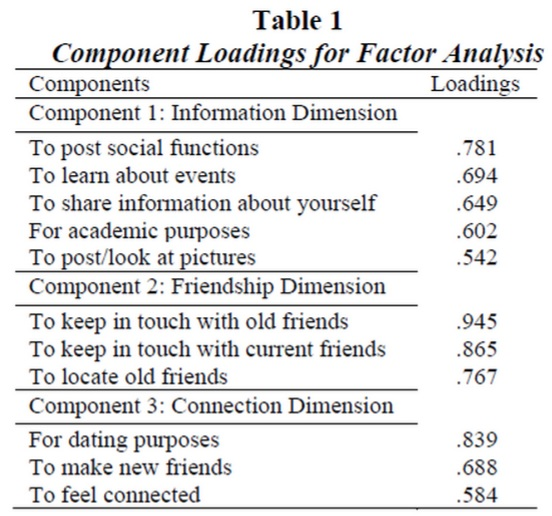
\includegraphics[width=90mm]{images/factoranalysis.jpg}
%	Figure 
%}
%\caption{Survey Results}
%\end{wrapfigure}

\begin{center}
  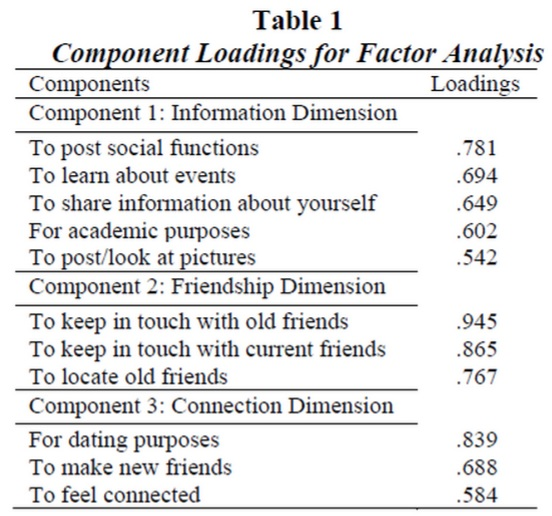
\includegraphics{images/factoranalysis.jpg}
  \captionof{figure}{Survey Results}
\end{center}

Some interesting correlations were found with further statistical analysis, for example; men significantly used social networks more for the purpose of sharing personal information and dating compared to women. While being somewhat more specific, these correlations are still slightly too generalised. However, this being said, knowing some of the more common reasons that people use Facebook will give us direction in terms of what types of feed objects we should be looking for.

Nad~\cite{nadkarni2012people} published a literature review which looked at user modelling Facebook users from a more psychological frame of view. They found that there were correlations between certain Facebook behavioural patterns and a uer's psychology. Some of the correlations that were found were:

\begin{itemize}
 \item Users with higher levels of extraversion tended to use Facebook as more of a social tool rather than to replace social activities. They also generally had accumulated more social networking friends  and had more addictive tendencies when it came to Facebook use 
 \item Users with higher levels of Neuroticism Levels tended to prefer reading information in their feed whereas users with lower levels of neuroticism preferred seeing photos
 \item Users with significantly high or low levels of neuroticism tend to be more open to share personal information on their profiles
\end{itemize}

These findings are closer to what we are looking for, however, it is not easy to determine the psychology of a user for the application of ranking their Facebook feed. However, once again, these results allow us to get a better idea of the different types of feed objects that are to be considered, for example information vs photos. 

It eventually became clear to us that even if we were to use these results for our user modelling, it is uncertain whether they are still relevant, as we saw, the survey conducted by Bon~\cite{bonds2010myspace} set out to confirm results from a study just 2 years previous to his research paper and already found that user's behaviour changed. So we began to look at how people perform user modelling and the practices involved with it. Cle~\cite{clemmensen2004four} conducted an interview with 4 different HCI proffessionals based in Sweden to gain insight into there methodologies and phylosophies. The following methods of performing user modelling that came from the interviews especially interested us and will most likely be used throughout our implementation:

\begin{itemize}
 \item Usability Tests - Observing how a user interacts with a system and asking good questions to extract meaningful feedback from the user.
 \item Surveying - Simply asking existing users questions that will aid us in our user modelling - as seen in the survey conducted by Bon~\cite{bonds2010myspace}
 \item Conceptualise how users are represented in the system (as data) - By thinking about how a user's preferences will be represented in the system itself, we are able to design our algorithms accordingly
 \item Creating personas and use cases/scenario - Designing a fictional character who would benefit from our system and creating a use case around it; this allows us to consider all the different types of users that can be modelled
\end{itemize}

With this information in mind, we have chosen to conduct another survey similar to the ones performed in the literature; to help deermine whether there are certain patterns in feed preferences for users and to group those patterns into user types. For example, if we find that there is a pattern of users that prefer to see friend's social updates, photo's and event information, we can classify those set of preferences as a user type. The survey questions will be formulated with ideas from the past surveys that have been conducted and will serve as the basis of our user modelling.

\section{Ranking Algorithms}

A ranking algorithm will give each item a score and order them with the item with the highest score at the top and the item with the lowest score at the bottom. The score of an item will depend on a set of criteria that the ranking algorithm uses. Social networking services will use these ranking algorithms in order to provide the user with items that will interest them. Since we are focusing on Facebook, the users will be provided with a feed that contains a lot of posts that they will receive. In Li~\cite{LiTiaLee2010} paper, they discovered that there are three major factors that could affect how interesting a user may find a particular item. They are:


\begin{itemize}
 \item Topical Preference
 \item Topological Locality
 \item Social Influence
\end{itemize}

Topical reference is the idea that most users are interested in a limited range of topics. Topological locality refers to the fact that users are interested in the topics that their friends like and Social influence basically says that users are interested in famous people such as singers or actors. These factors do provide some insight on what a user likes but could be further generalised to topics that a user likes. The Topological locality does raise an interesting notion, that is, users are more likely to like a post that a friend likes. We can summarize these two into a more general categorization of Topic classification and connections. Topic classification will be classifying the topics that a user may like while connections will be a measure of how 'close' the user is with their friend based on their interactivity. 

Topic classification is quite difficult we have to generalise a topic that they may like based on the posts that they receive. In a paper by Bur~\cite{Bur2013}, they analysed twitter tweets and tried to generalise a topic based on the tweets each user received. They have analysed two types of methods. They are:
\begin{itemize}
 \item BestOverlap
 \item UserInfoBigram
\end{itemize}

The BestOverlap method attempts to gather a huge amount of tweets and look at the common words in those tweets. A topic can be generated by the word is overlapped the most across all the tweets. In regards to our algorithm where we have to look at Facebook posts, the likelihood of word overlaps across a large amount of posts is quite low. This method would not be appropriate for our purposes.

The UserInfoBigram analyses the optional text that is provided in every tweet and generalises a topic from those words. In Facebook, almost no one uses the optional text so this method will also not work.

In order to do topic classificication we had to look to a paper by Szo~\cite{szomszor2008semantic} who proposed a system for defining topics of interest with the aid of Wikipedia. He collated a list of tags using a user's "tagging activity" which, for our purposes could mean commonly used words in past posts. These tags are then verified using Wikipedia to check that there indeed does exist something along the lines of the tag. Wikipedia is chosen over more formal dictionaries due the the nature of social media tags not being real words, thus many of the tags will not be able to be verified by formal dictionaries such as WordNet. Wikipedia is then traversed (from the tag's wiki page) to find a super category that the tag belongs to. For example if a user generates the tag "C++", in Wikipedia, the C++ page is a subpage of the "Programming Language Families" page. 
Since a single verified tag can have many categories and the final list ends up being dominated by the broader categories, only categories that meet either of these criteria are taken:
\begin{itemize}
 \item The tag has only 1 category
 \item The category matches the tag name exactly
 \item The category is a plural of the tag
\end{itemize}

This approach nets us a list of the users general interests, which can then be used to determine how much a certain post is related to the user's interests by observing the contents of the post and determining if they belong to any of these topics, again using Wikipedia.

Aga~\cite{Aga2014} discusses activity ranking for LinkedIn which is also a Social Networking Service. They discover two more factors that have a huge impact on whether the activity is deemed interesting or not. They used the measurement of CTR or click-through-rate which is the probability of a user clicking on the link to measure the appeal of an activity. An activity that was old had a low CTR compared to an activity that was new. It seems that the freshness of an activity or the time that the activity was made had to be taken into account in the ranking algorithm. Another factor was diversity. A huge drop in CTR was found when they gave users a repeated type of activity in their feed. We can surmise that freshness and diversity are key factors that must be considered in our ranking algorithm. The method that they have used to deal with these two issues involved re-ranking the feed with a decay factor to account for time and adding a negative score to activities of the same type. For our algorithm, we plan to utilise the same methods proposed as they have been successful.

Aga~\cite{Aga2014} also reinforces the idea that people are interested in what their friends like when they analysed the activities of co-workers and colleagues. Like Li~\cite{LiTiaLee2010}, they found that there was an increase in the click-through-rate of activities they were made by co-workers in the same organisation and colleagues. This emphasizes the importance of the factor of connections.
